%%%%%%%%%%%%%%%%%%%%%%%%%%%%%%%%%%%%%%%%%%%%%%%%%%%%%%%%%%%%%%%%%%%%%%%%%%%%%%%%%%%%%%%%%%%%%%%%%%%%%%%%%%%%%%%
\begin{landscape}
\chapter{Přehled parametrů jednotlivých jednodeskových počítačů}
\label{PrilohaTabulkaTabulka}
\centering
\vspace{5pt}
\resizebox{\paperwidth}{!}{%
\begin{tabular}{|c|c|c|c|c|c|c|c|c|c|c|c|c|c|c|c|c|c|c|c|c|c|c|c|c|c|}
\hline

\rotatebox[origin=c]{90}{\parbox[b]{4cm}{\hspace{10pt}\textbf{Výrobce desky}}} &                        
\rotatebox[origin=c]{90}{\parbox[b]{4cm}{\hspace{10pt}\textbf{Označení modelu}}} & 
\rotatebox[origin=c]{90}{\parbox[b]{4cm}{\hspace{10pt}\textbf{Mikrokontrolér}}} & 
\rotatebox[origin=c]{90}{\parbox[b]{4cm}{\hspace{10pt}\textbf{Platforma}}} & 
\rotatebox[origin=c]{90}{\parbox[b]{4cm}{\hspace{10pt}\textbf{Frekvence}}} & 
\rotatebox[origin=c]{90}{\parbox[b]{4cm}{\hspace{10pt}\textbf{Flash [KiB]}}} & 
\rotatebox[origin=c]{90}{\parbox[b]{4cm}{\hspace{10pt}\textbf{EEPROM [KiB]}}} & 
\rotatebox[origin=c]{90}{\parbox[b]{4cm}{\hspace{10pt}\textbf{RAM [KiB]}}} & 
\rotatebox[origin=c]{90}{\parbox[b]{4cm}{\hspace{10pt}\textbf{Digitální piny}}} &
\rotatebox[origin=c]{90}{\parbox[b]{4cm}{\hspace{10pt}\textbf{PWM kanály}}} &
\rotatebox[origin=c]{90}{\parbox[b]{4cm}{\hspace{10pt}\textbf{Analogové vstupy}}} & 
\rotatebox[origin=c]{90}{\parbox[b]{4cm}{\hspace{10pt}\textbf{UART sběrnice}}} &
\rotatebox[origin=c]{90}{\parbox[b]{4cm}{\hspace{10pt}\textbf{I2C sběrnice}}} &
\rotatebox[origin=c]{90}{\parbox[b]{4cm}{\hspace{10pt}\textbf{SPI sběrnice}}} &
\rotatebox[origin=c]{90}{\parbox[b]{4cm}{\hspace{10pt}\textbf{Ethernet}}} &
\rotatebox[origin=c]{90}{\parbox[b]{4cm}{\hspace{10pt}\textbf{Wi-Fi}}} &
\rotatebox[origin=c]{90}{\parbox[b]{4cm}{\hspace{10pt}\textbf{USB master}}} &
\rotatebox[origin=c]{90}{\parbox[b]{4cm}{\hspace{10pt}\textbf{MicroSD}}} &
\rotatebox[origin=c]{90}{\parbox[b]{4cm}{\hspace{10pt}\textbf{Mini PCI-e}}} &
\rotatebox[origin=c]{90}{\parbox[b]{4cm}{\hspace{10pt}\textbf{SATA}}} &
\rotatebox[origin=c]{90}{\parbox[b]{4cm}{\hspace{10pt}\textbf{Grafický výstup}}} &
\rotatebox[origin=c]{90}{\parbox[b]{4cm}{\hspace{10pt}\textbf{Bluetooth}} }&
\rotatebox[origin=c]{90}{\parbox[b]{4cm}{\hspace{10pt}\textbf{HDMI}}} &
\rotatebox[origin=c]{90}{\parbox[b]{4cm}{\hspace{10pt}\textbf{Podpora shieldů}} }&
\rotatebox[origin=c]{90}{\parbox[b]{4cm}{\hspace{10pt}\textbf{USB rozhraní}}} &
\rotatebox[origin=c]{90}{\parbox[b]{4cm}{\hspace{10pt}\textbf{Rozměry}}} \\ \hline \hline



\multirow{13}{*}{\textbf{Arduino}}        & \textbf{Diecimila}              & ATmega168                & ARM       & 16 MHz              & 16              & 0.5              & 1              & 14             & 6          & 6                & ano           & ano          & ano          & ne       & ne   & ne         & ne      & ne        & ne   & ne              & ne        & ne   & ano             & FTDI          & 68.6 x 53.3 mm   \\ \cline{2-26}
                & \textbf{Duemilanove (v2)}       & ATmega328P               & ARM       & 16 MHz              & 32              & 1                & 2              & 14             & 6          & 6                & ano           & ano          & ano          & ne       & ne   & ne         & ne      & ne        & ne   & ne              & ne        & ne   & ano             & FTDI          & 68.6 x 53.3 mm   \\ \cline{2-26} 
                & \textbf{Uno (R3)}               & ATmega328P               & ARM       & 16 MHz              & 32              & 1                & 2              & 14             & 6          & 6                & ano           & ano          & ano          & ne       & ne   & ne         & ne      & ne        & ne   & ne              & ne        & ne   & ano             & ATmega8U2     & 68.6 x 53.3 mm   \\ \cline{2-26} 
                & \textbf{Due}                    & ATMEL SAM3U              & ARM       & 84 MHz              & 512             & 1                & 96             & 54             & 12         & 16               & ano           & ano          & ano          & ne       & ne   & ne         & ne      & ne        & ne   & ne              & ne        & ne   & ano             & Prog + Native & 101.5 x 53.3 mm  \\ \cline{2-26}
                & \textbf{Mega (2560)}            & ATmega2560               & ARM       & 16 MHz              & 256             & 4                & 8              & 54             & 14         & 16               & ano           & ano          & ano          & ne       & ne   & ne         & ne      & ne        & ne   & ne              & ne        & ne   & ano             & FTDI          & 101.5 x 53.3 mm  \\ \cline{2-26}
                & \textbf{Leonardo}              & ATmega32u4               & ARM       & 16 MHz              & 32              & 1                & 2              & 14             & 6          & 12               & ano           & ano          & ano          & ne       & ne   & ne         & ne      & ne        & ne   & ne              & ne        & ne   & ano             & Atmega32u4    & 68.6 × 53.3mm    \\ \cline{2-26}
                & \textbf{Fio}                   & ATmega328P               & ARM       & 8 MHz               & 32              & 1                & 2              & 14             & 6          & 8                & ano           & ano          & ano          & ne       & ne   & ne         & ne      & ne        & ne   & ne              & ne        & ne   & ne              & FTDI          & 40.6 x 27.9 mm   \\ \cline{2-26}
                & \textbf{Mini}                  & ATmega328P               & ARM       & 16 MHz              & 32              & 1                & 2              & 14             & 6          & 8                & ano           & ano          & ano          & ne       & ne   & ne         & ne      & ne        & ne   & ne              & ne        & ne   & ne              & UART          & 30.5 x 18.0 mm   \\ \cline{2-26}
                & \textbf{Micro}                  & ATmega32u4               & ARM       & 16 MHz              & 32              & 1                & 2.5            & 20             & 7          & 12               & ano           & ano          & ano          & ne       & ne   & ne         & ne      & ne        & ne   & ne              & ne        & ne   & ne              & Atmega32u4    & 50.0 x 13.0 mm   \\ \cline{2-26}
                & \textbf{Nano v2}               & ATmega328                & ARM       & 16 MHz              & 32              & 1                & 2              & 14             & 6          & 8                & ano           & ano          & ano          & ne       & ne   & ne         & ne      & ne        & ne   & ne              & ne        & ne   & ne              & FTDI          & 43.0 x 18.0 mm   \\ \cline{2-26}
                & \textbf{LilyPad (v2)}           & ATmega328V               & ARM       & 8 MHz               & 16              & 0.5              & 1              & 14             & 6          & 6                & ano           & ne           & ne           & ne       & ne   & ne         & ne      & ne        & ne   & ne              & ne        & ne   & ne              & UART          & ø 50mm           \\ \cline{2-26}
                & \multirow{2}{*}{\textbf{Ýun}}                    & Atheros AR9331           & x86       & 400 MHz             & 16 MiB          & \multirow{2}{*}{1}                & 64 MB          & \multirow{2}{*}{-}               & \multirow{2}{*}{7}           & \multirow{2}{*}{12}               & \multirow{2}{*}{ano}            & \multirow{2}{*}{ano}           & \multirow{2}{*}{ano}           & \multirow{2}{*}{ano}       & \multirow{2}{*}{ano}  & \multirow{2}{*}{ano}         & \multirow{2}{*}{ano}      & \multirow{2}{*}{ne}         & \multirow{2}{*}{ne}   & \multirow{2}{*}{ne}               & \multirow{2}{*}{ne}         & \multirow{2}{*}{ne}    & \multirow{2}{*}{ano}             & \multirow{2}{*}{Atmega32u4}    & \multirow{2}{*}{68.6 x 53.3 mm}    \\ \cline{3-6} \cline{8-8}
                &                        & ATmega32u4               & ARM       & 16 MHz              & 32              &                  & 1              &                &            &                  &               &              &              &          &      &            &         &           &      &                 &           &      &                 &               &                  \\ \hline
\multirow{10}{*}{\textbf{Arduino klony}}   & \textbf{Teensy (v 3.2)}         & MK20DX256                & ARM       & 72 MHz              & 256             & 64               & 2              & 34             & 21         & 1                & ano           & ano          & ano          & ne       & ne   & ne         & ne      & ne        & ne   & ne              & ne        & ne   & ne              & FTDI          & 30.5 x 18.0 mm   \\ \cline{2-26}
                & \textbf{Freeduino }             & ATmega168                & ARM       & 16 MHz              & 16              & 0.5              & 1              & 14             & 6          & 6                & ano           & ano          & ano          & ne       & ne   & ne         & ne      & ne        & ne   & ne              & ne        & ne   & ano             & FTDI          & 68.6 x 53.3 mm   \\ \cline{2-26}
                & \textbf{LABduino }              & ATmega328P               & ARM       & 16 MHz              & 32              & 1                & 2              & 14             & 6          & 6                & ano           & ano          & ano          & ne       & ne   & ne         & ne      & ne        & ne   & ne              & ne        & ne   & ano             & FTDI          & 51.0 x 51.0 mm   \\ \cline{2-26}
                & \textbf{Arduelo Libero}         & ATmega168                & ARM       & 16 MHz              & 16              & 0.5              & 1              & 14             & 6          & 6                & ano           & ano          & ano          & ne       & ne   & ne         & ne      & ne        & ne   & ne              & ne        & ne   & ano             & FTDI          & 68.6 x 53.3 mm   \\ \cline{2-26}
                & \textbf{Bare Bones Board }      & ATmega328P               & ARM       & 16 MHz              & 32              & 1                & 2              & 20             & 6          & 6                & ano           & ano          & ano          & ne       & ne   & ne         & ne      & ne        & ne   & ne              & ne        & ne   & ne              & FTDI          & 59.7 x 40.6 mm   \\ \cline{2-26}
                & \textbf{Nanode}                 & ATmega328P               & ARM       & 16 MHz              & 32              & 1                & 2              & 14             & 6          & 6                & ano           & ano          & ano          & ne       & ne   & ne         & ne      & ne        & ne   & ne              & ne        & ne   & ano             & ATmega8U2     & 68.6 x 53.3 mm   \\ \cline{2-26}
                & \textbf{Freaduino}              & ATmega328P               & ARM       & 16 MHz              & 32              & 1                & 2              & 14             & 6          & 6                & ano           & ano          & ano          & ne       & ne   & ne         & ne      & ne        & ne   & ne              & ne        & ne   & ano             & ATmega8U2     & 68.6 x 53.3 mm   \\ \cline{2-26}
                & \textbf{Seeeduino }             & ATmega1280               & ARM       & 16 MHz              & 128             & 4                & 8              & 54             & 14         & 16               & ano           & ano          & ano          & ne       & ne   & ne         & ne      & ne        & ne   & ne              & ne        & ne   & ano             & FTDI          & 68.6 x 53.3 mm   \\ \cline{2-26}
                & \textbf{Diavolino }             & ATmega328P               & ARM       & 16 MHz              & 32              & 1                & 2              & 14             & 6          & 6                & ano           & ano          & ano          & ne       & ne   & ne         & ne      & ne        & ne   & ne              & ne        & ne   & ano             & ATmega8U2     & 68.6 x 53.3 mm   \\ \cline{2-26}
                & \textbf{Boarduino}              & ATmega328P               & ARM       & 16 MHz              & 16              & 0.5              & 1              & 14             & 6          & 6                & ano           & ano          & ano          & ne       & ne   & ne         & ne      & ne        & ne   & ne              & ne        & ne   & ano             & FTDI          & 75.0 x 20.0 mm   \\  \hline
\multirow{2}{*}{\textbf{Intel}}            & \textbf{Galileo}                & Intel Quark X1000        & x86       & 400 MHz             & 8 MB            & 8                & 256 MB         & 14             & 6          & 6                & ano           & ano          & ano          & ano      & ne   & ano        & ano     & ano       & ne   & ano             & ne        & ne   & ano             & 2 x USB       & 123.8 x 72.0 mm  \\ \cline{2-26} 
                & \textbf{Edison}                 & Intel Atom + Intel Quark & x86       & 500 MHz             & 4 GB            & 8                & 1 GB           & 20             & 4          & 6                & ano           & ano          & ano          & ne       & ano  & ano        & ano     & ne        & ne   & ne              & ano       & ne   & ano             & dle desky     & 35.5 x 25.0 mm   \\  \hline
\multirow{2}{*}{\textbf{AMD}}            & \textbf{Gizmo 1}                & AMD GX210HA              & amd64     & 1 GHz               & ne              & -                & 1 GB           & ano            & ano        & ano              & ano           & ano          & ano          & ano      & ne   & ano        & ano     & ne        & ano  & ano             & ne        & ne   & ne              & 2x USB        & 101.6 x 101.6 mm \\ \cline{2-26} 
                & \textbf{Gizmo 2}                & AMD GX210HA              & amd64     & 1 GHz               & ne              & -                & 1 GB           & ano            & ano        & ano              & ano           & ano          & ano          & ano      & ne   & ano        & ano     & ano       & ano  & ano             & ne        & ano  & ne              & 2x USB        & 101.6 x 101.6 mm \\  \hline
\multirow{6}{*}{\textbf{Raspberry}}       & \textbf{Raspbery Pi A+  }       & Broadcom ARM 1176        & ARM       & 700 MHz             & ne              & -                & 256 MB         & 8              & 1          & ne               & ano           & ano          & ano          & ne       & ne   & ano        & ano     & ne        & ne   & ano             & ne        & ano  & ano             & 1x USB SoC    & 65.0 x 56.0 mm   \\ \cline{2-26} 
                & \textbf{Raspbery Pi B }         & Broadcom BCM 2835        & ARM       & 700 MHz             & ne              & -                & 512 MB         & 8              & 1          & ne               & ano           & ano          & ano          & ano      & ne   & ano        & SD      & ne        & ne   & ano             & ne        & ano  & ano             & 4x USB SoC    & 85.6 x 53.98 mm  \\ \cline{2-26}
                & \textbf{Raspbery Pi B+}         & Broadcom BCM 2835        & ARM       & 700 MHz             & ne              & -                & 512 MB         & 13             & 1          & ne               & ano           & ano          & ano          & ano      & ne   & ano        & ano     & ne        & ne   & ano             & ne        & ano  & ano             & 4x USB SoC    & 85 x 56 x 17 mm  \\ \cline{2-26}
                & \textbf{Raspbery Pi 2 }         & Broadcom BCM 2836        & ARM       & 900 MHz             & ne              & -                & 1 GB           & 13             & 1          & ne               & ano           & ano          & ano          & ano      & ne   & ano        & ano     & ne        & ne   & ano             & ne        & ano  & ano             & 4x USB SoC    & 86 x 56 x 17 mm  \\ \cline{2-26}
                & \textbf{Raspbery Pi 3 }         & Broadcom BCM 2837        & ARM       & 1.2 Ghz             & ne              & -                & 1 GB           & 13             & 1          & ne               & ano           & ano          & ano          & ano      & ano  & ano        & ano     & ne        & ne   & ano             & ne        & ano  & ano             & 4x USB SoC    & 87 x 56 x 17 mm  \\ \cline{2-26}
                & \textbf{Raspbery Pi Zero }      & Broadcom BCM 2835        & ARM       & 1 GHz               & ne              & -                & 512 MB         & 13             & 1          & ne               & ano           & ano          & ano          & ne       & ano  & ano        & ano     & ne        & ne   & ano             & ano       & ano  & ano             & 1x USB SoC    & 65  x 30  x 5 mm \\  \hline
\multirow{7}{*}{\textbf{Raspberry klony}}  & \textbf{Banana Pi (M3) }        & Allwinner A83T           & ARM       & 1.8 GHz             & 8 GB            & -                & 2 GB           & 13             & 1          & ne               & ano           & ano          & ano          & ano      & ano  & ano        & ano     & ne        & ano  & ano             & ano       & ano  & ano             & 2x USB SoC    & 92.0 x 60.0 mm   \\ \cline{2-26}
                & \textbf{OrangePi (+2) }         & Allwinner H3             & ARM       & 1.6 GHz             & 16 GB           & -                & 2 GB           & 13             & 1          & ne               & ano           & ano          & ano          & ano      & ano  & ano        & ano     & ne        & ano  & ano             & ano       & ano  & ano             & 4x USB SoC    & 108 × 67.0 mm    \\ \cline{2-26}
                & \textbf{CubieBoard (v5) }       & Allwinner H8             & ARM       & 2 GHz               & 8 GB            & -                & 2 GB           & ano            & ano        & ne               & ano           & ano          & ano          & ano      & ano  & ano        & ano     & ano       & ano  & ano             & ano       & ano  & ano             & 3x USB SoC    & 110 x 80 mm      \\ \cline{2-26}
                & \textbf{UpBoard (v1)}           & Intel X5-Z8350           & ARM       & 1.92 GHz            & 64 GB           & -                & 4 GB           & ano            & ano        & ne               & ano           & ano          & ano          & ano      & ne   & ano        & ne      & ne        & ne   & ano             & ne        & ano  & ne              & 4x USB SoC    & 85.6  × 56.5 mm  \\ \cline{2-26}
                & \textbf{PINE64 (+2)}            & Cortex A53               & ARM       & 1.2 GHz             & ne              & -                & 2 GB           & ano            & ano        & ano              & ano           & ano          & ano          & ano      & ano  & ano        & ano     & ne        & ne   & ano             & ano       & ano  & ano             & 2x USB SoC    & 127 x 79 mm      \\ \cline{2-26}
                & \textbf{HardKernel Odroid (C2)} & Amlogic S905             & ARM       & 1.5 GHz             & ne              & -                & 2 GB           & ano            & ano        & ne               & ano           & ano          & ano          & ano      & ne   & ano        & ano     & ano       & ne   & ano             & ne        & ano  & ano             & 4x USB SoC    & 85.0 x 56.0 mm   \\ \cline{2-26}
                & \textbf{BeagleBoard (Black)}    & Sitara AM3358/9          & ARM       & 1 GHz               & 2 GB            & -                & 512 MB         & ano            & 8          & ano              & 4             & ano          & ano          & ano      & ano  & ano        & ano     & ne        & ne   & ano             & ano       & ano  & ano             & 2x USB SoC    & 86.4 x 53.3 mm   \\  \hline  \hline
\end{tabular}}

\end{landscape}

%%%%%%%%%%%%%%%%%%%%%%%%%%%%%%%%%%%%%%%%%%%%%%%%%%%%%%%%%%%%%%%%%%%%%%%%%%%%%%%%%%%%%%%%%%%%%%%%%%%%%%%%%%%%%%%
%\chapter{Vývojový diagram aplikace pro vyčítání dat}
%\label{AplikaceDiagram}
%\vspace{-20pt}
% \begin{figure}[!ht]
%  \begin{center}
%    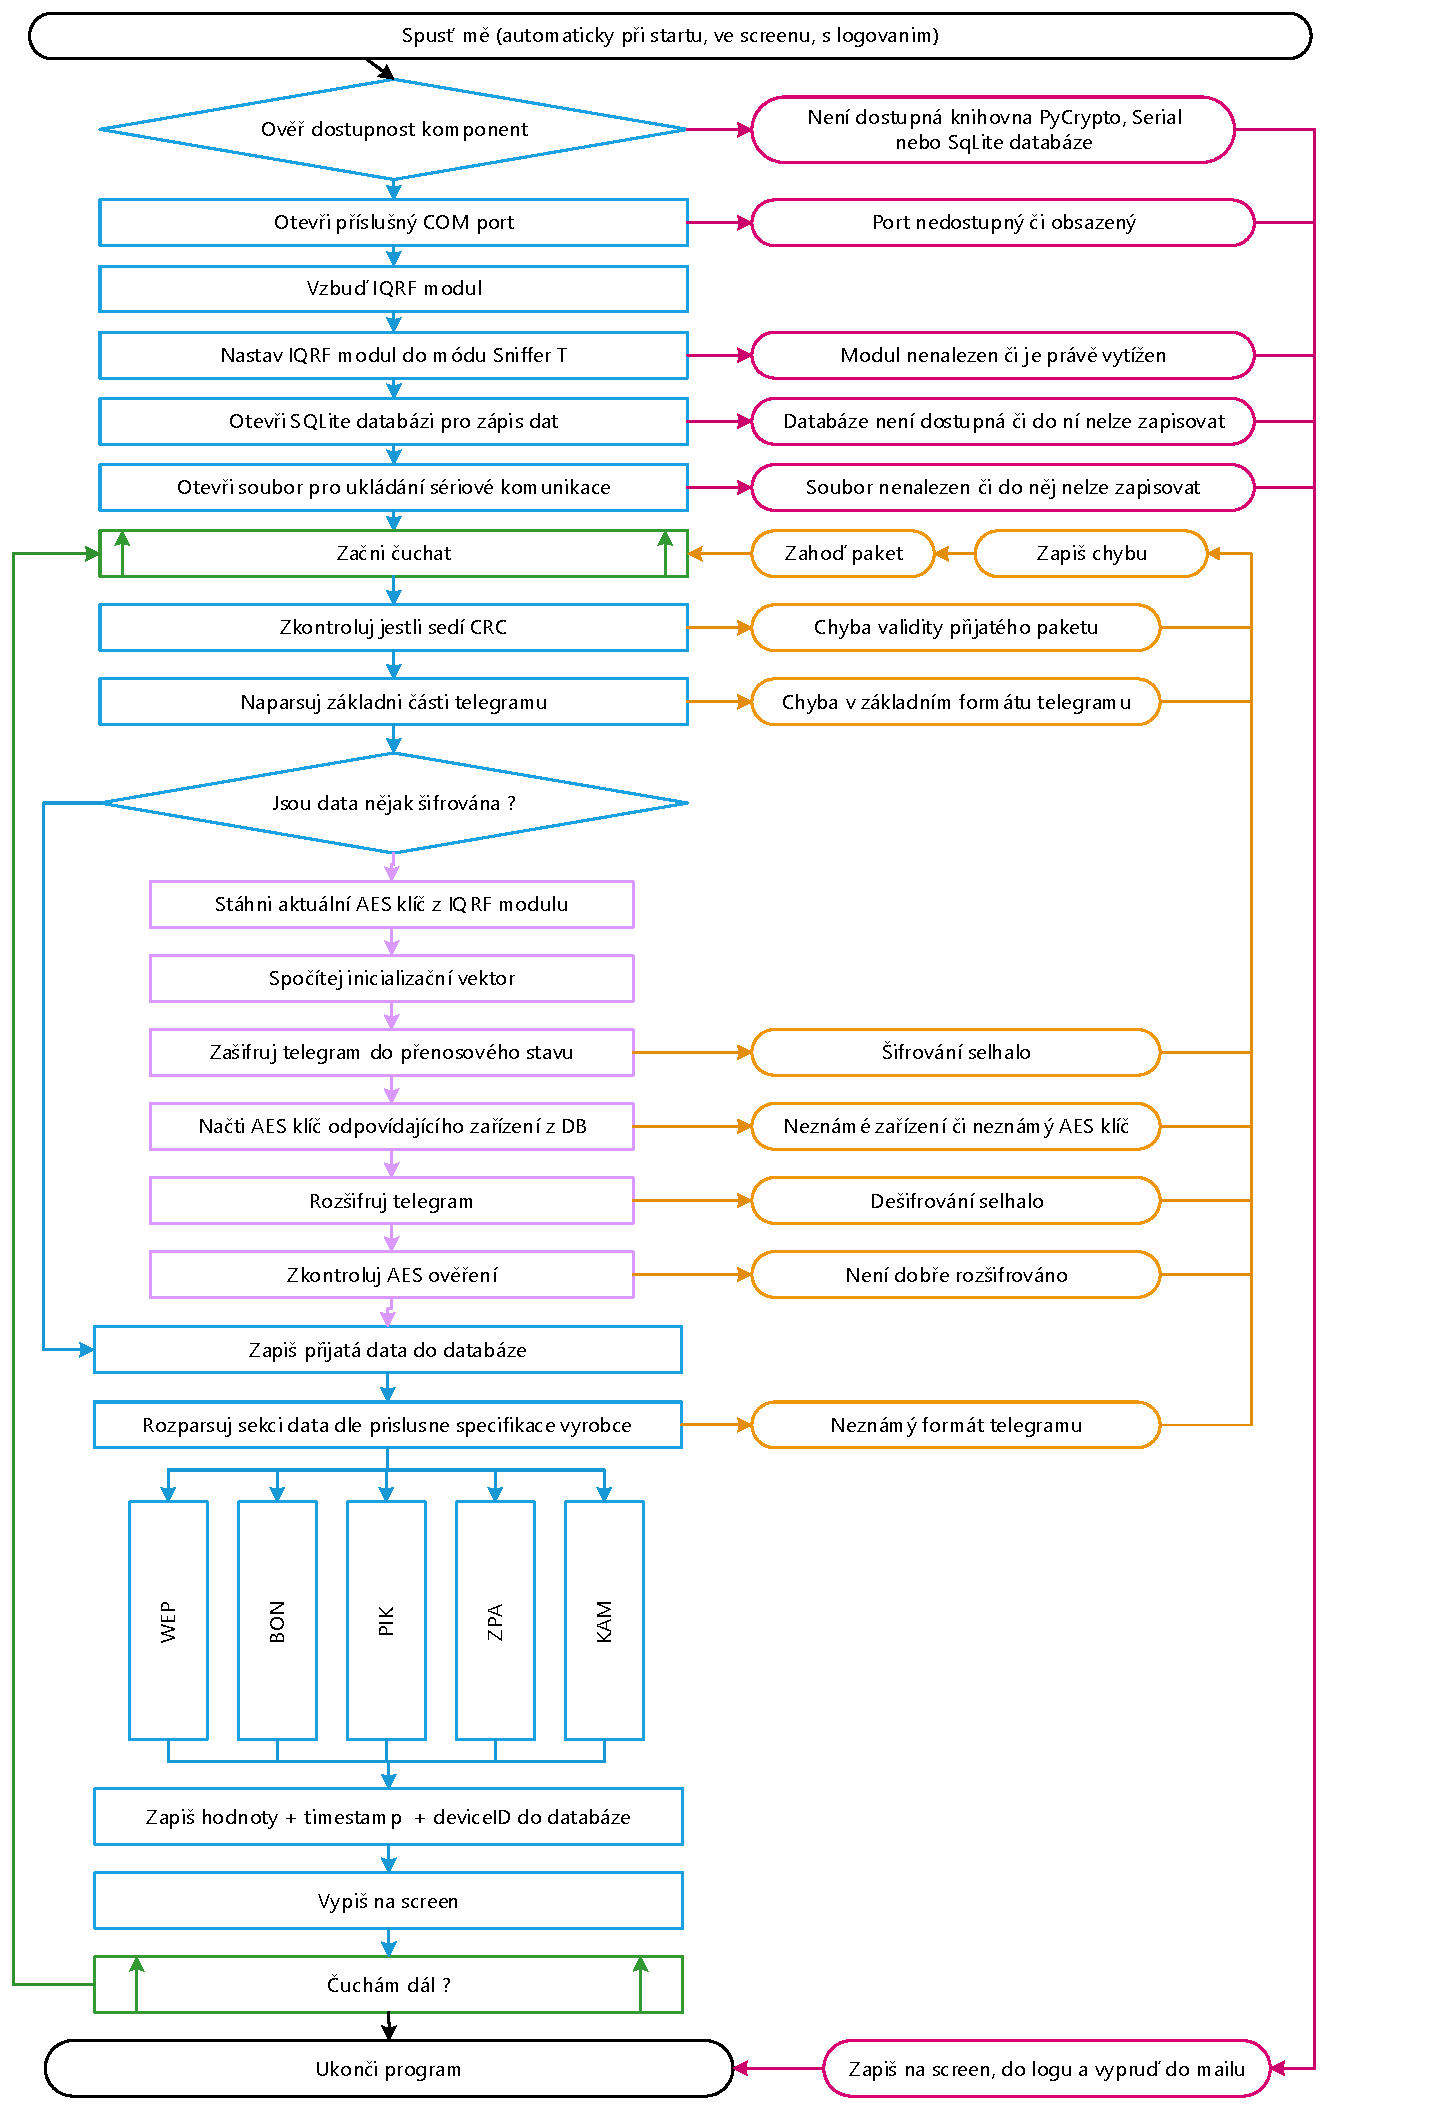
\includegraphics[scale=0.55]{obrazky/aplikace_diagram}
%  \end{center}
%\end{figure}

%%%%%%%%%%%%%%%%%%%%%%%%%%%%%%%%%%%%%%%%%%%%%%%%%%%%%%%%%%%%%%%%%%%%%%%%%%%%%%%%%%%%%%%%%%%%%%%%%%%%%%%%%%%%%%%
\begin{landscape}
\chapter{Ukázka zachycených dat}
\label{PrilohaVystup}
	\begin{lstlisting}[style=MyCodeC]
19/04/2017 20:47:48  Running in: Real sniffer mode.
19/04/2017 20:47:48  Device is on AMA0: True
19/04/2017 20:47:49  Device is waked up: OK
19/04/2017 20:47:50  Device is set as Sniffer T: OK
19/04/2017 20:47:51  Default AES key set: OK
19/04/2017 20:47:51  Sniffing now:
19/04/2017 20:48:14  AccNo: 181  Device: BON.06.00000121.01  RSSI: -49.5dB  AES: True   Volume: 31567l 		
19/04/2017 20:48:46  AccNo: 182  Device: BON.07.00000121.01  RSSI: -49.5dB  AES: True   Volume: 28678l 
19/04/2017 20:48:47  AccNo: 203  Device: WEP.1b.00000010.02  RSSI: -40.0dB  AES: True   Temperature: 20.4C  Humidity: 35.1%
19/04/2017 20:49:12  AccNo:  71  Device: ZPA.02.01754247.01  RSSI: -74.5dB  AES: False  Tariff1: 3.0kWh  Tariff2: 11.0kWh
19/04/2017 20:49:19  AccNo: 182  Device: BON.06.00000121.01  RSSI: -49.5dB  AES: True   Volume: 31567l 
19/04/2017 20:49:48  AccNo: 204  Device: WEP.1b.00000010.02  RSSI: -40.0dB  AES: True   Temperature: 20.4C  Humidity: 35.0%		
19/04/2017 20:49:49  AccNo: 183  Device: BON.07.00000121.01  RSSI: -49.0dB  AES: True   Volume: 28678l
19/04/2017 20:50:12  AccNo:  71  Device: ZPA.02.01754247.01  RSSI: -74.0dB  AES: False  Tariff1: 3.0kWh  Tariff2: 11.0kWh
19/04/2017 20:50:18  AccNo: 183  Device: BON.06.00000121.01  RSSI: -49.0dB  AES: True   Volume: 31567l
19/04/2017 20:50:48  AccNo: 205  Device: WEP.1b.00000010.02  RSSI: -40.0dB  AES: True   Temperature: 20.4C  Humidity: 35.2%
19/04/2017 20:50:50  AccNo: 184  Device: BON.07.00000121.01  RSSI: -49.0dB  AES: True   Volume: 28678l
19/04/2017 20:51:12  AccNo:  71  Device: ZPA.02.01754247.01  RSSI: -74.0dB  AES: False  Tariff1: 3.0kWh  Tariff2: 11.0kWh
19/04/2017 20:51:22  AccNo: 184  Device: BON.06.00000121.01  RSSI: -49.0dB  AES: True   Volume: 31567l
19/04/2017 20:51:48  AccNo: 206  Device: WEP.1b.00000010.02  RSSI: -40.0dB  AES: True   Temperature: 20.4C  Humidity: 35.0%
19/04/2017 20:51:52  AccNo: 185  Device: BON.07.00000121.01  RSSI: -49.0dB  AES: True   Volume: 28678l
19/04/2017 20:52:12  AccNo:  71  Device: ZPA.02.01754247.01  RSSI: -74.0dB  AES: False  Tariff1: 3.0kWh  Tariff2: 11.0kWh
19/04/2017 20:52:24  AccNo: 185  Device: BON.06.00000121.01  RSSI: -49.0dB  AES: True   Volume: 31567l 
19/04/2017 20:52:49  AccNo: 207  Device: WEP.1b.00000010.02  RSSI: -40.0dB  AES: True   Temperature: 20.4C  Humidity: 34.9%
19/04/2017 20:52:52  AccNo: 186  Device: BON.07.00000121.01  RSSI: -49.0dB  AES: True   Volume: 28678l
19/04/2017 20:53:12  AccNo:  71  Device: ZPA.02.01754247.01  RSSI: -74.0dB  AES: False  Tariff1: 3.0kWh  Tariff2: 11.0kWh
	\end{lstlisting}
\end{landscape}
	
%%%%%%%%%%%%%%%%%%%%%%%%%%%%%%%%%%%%%%%%%%%%%%%%%%%%%%%%%%%%%%%%%%%%%%%%%%%%%%%%%%%%%%%%%%%%%%%%%%%%%%%%%%%%%%%
\begin{landscape}
\chapter{Ukázka vizualizace dat}
\label{PrilohaGrafy}
	 \begin{figure}[!ht]
  \begin{center}
    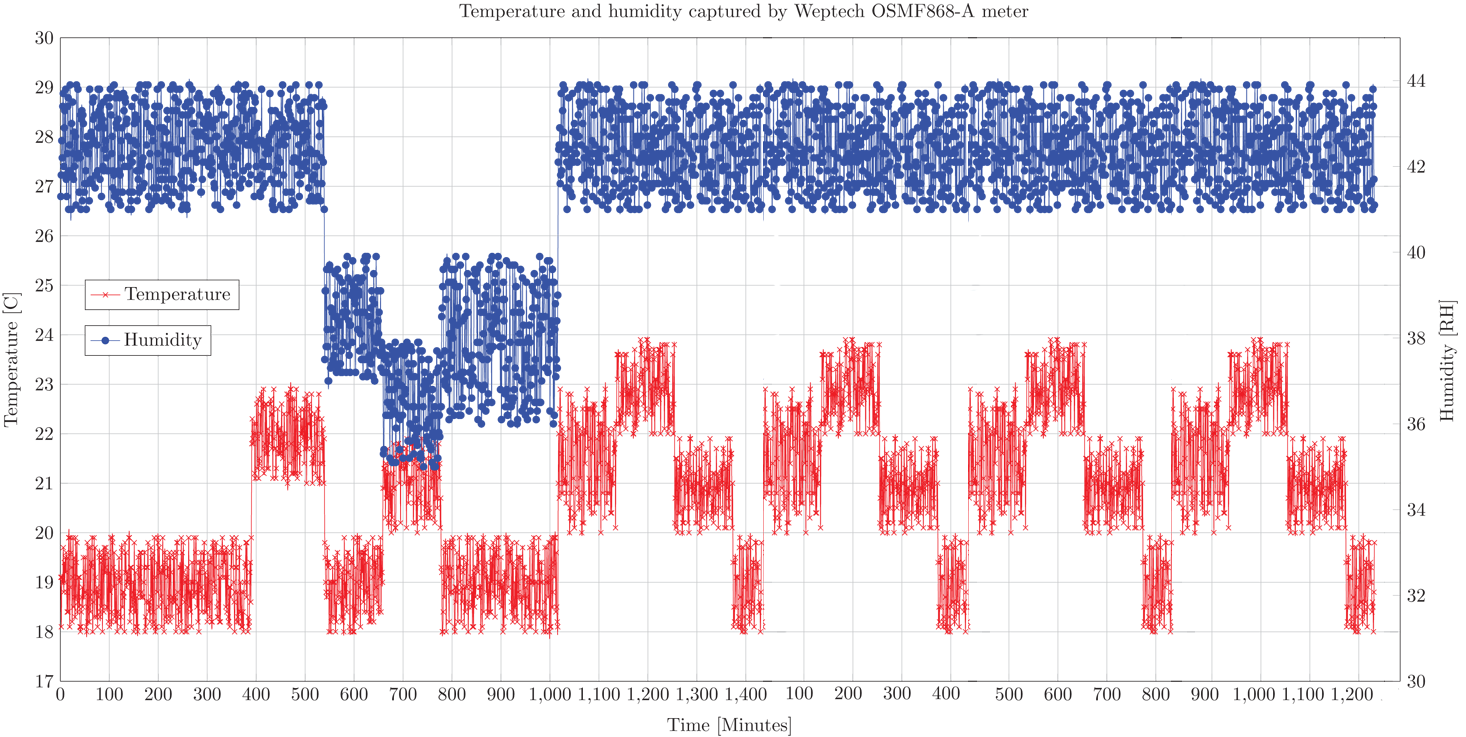
\includegraphics[scale=1.8]{obrazky/chart_weptech}
  \end{center}
  \caption{Vizualizace měření čidlem Weptech}
	\label{GrafPriloha1}
\end{figure}
	 \begin{figure}[!ht]
  \begin{center}
    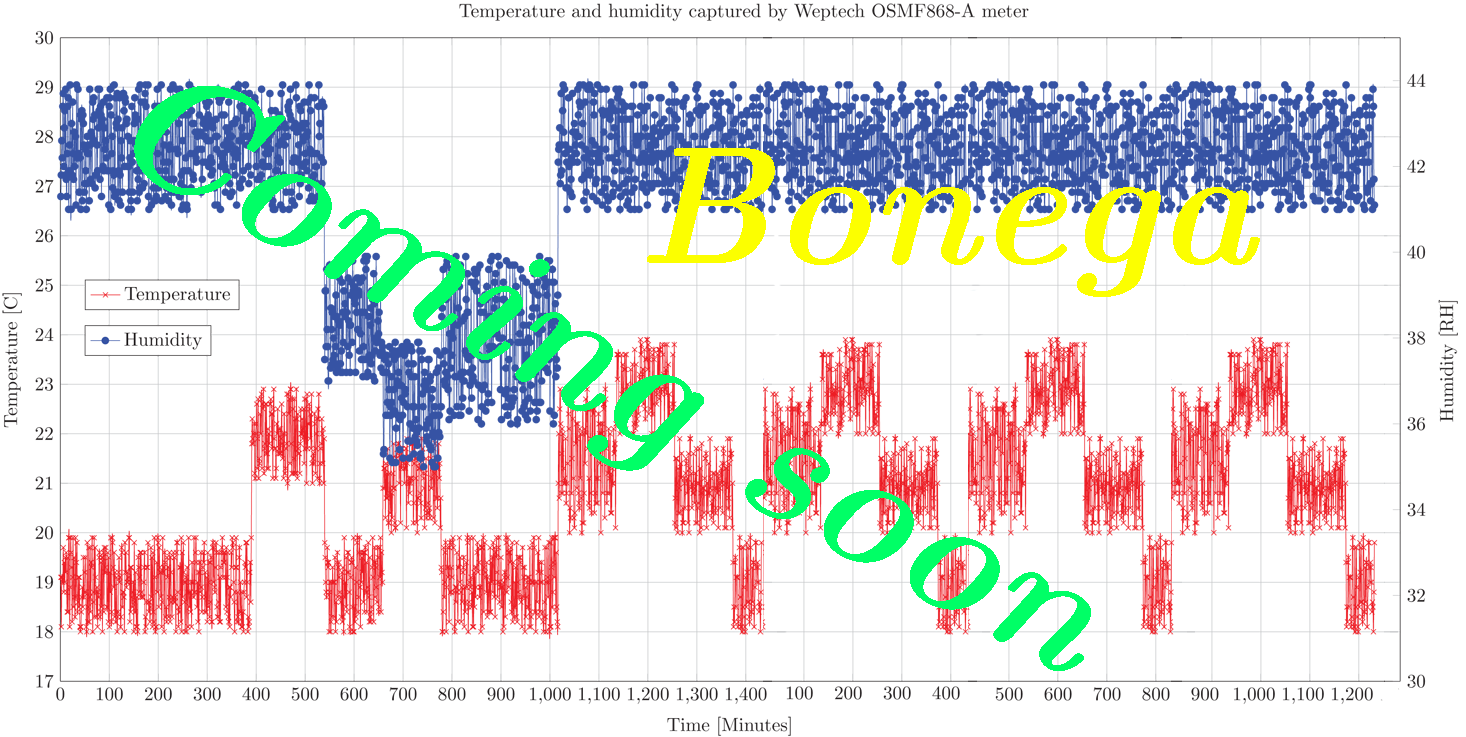
\includegraphics[scale=1.8]{obrazky/chart_bonega}
  \end{center}
  \caption{Vizualizace měření čidly Bonega}
	\label{GrafPriloha2}
\end{figure}
	 \begin{figure}[!ht]
  \begin{center}
    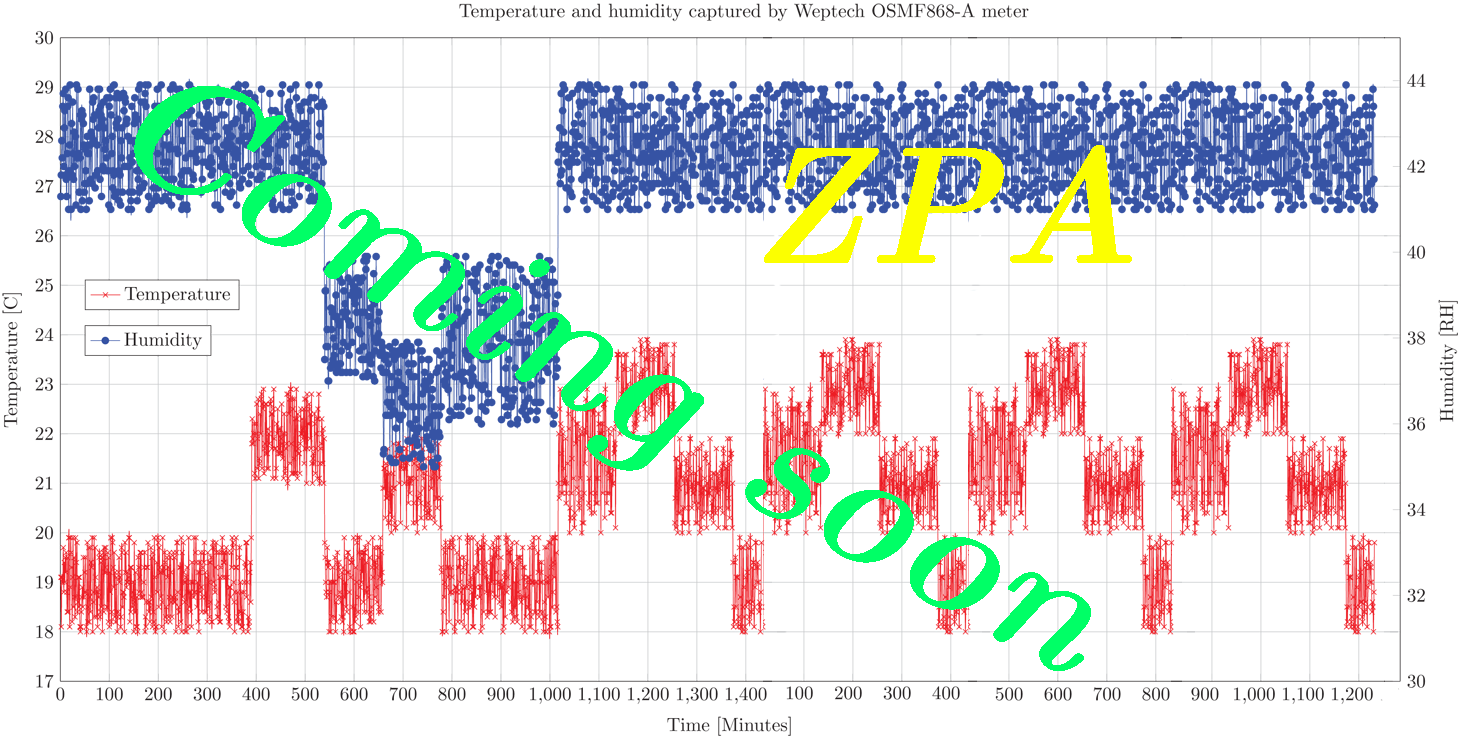
\includegraphics[scale=1.8]{obrazky/chart_zpa}
  \end{center}
  \caption{Vizualizace měření elektroměrem ZPA}
	\label{GrafPriloha3}
\end{figure}
	 \begin{figure}[!ht]
  \begin{center}
    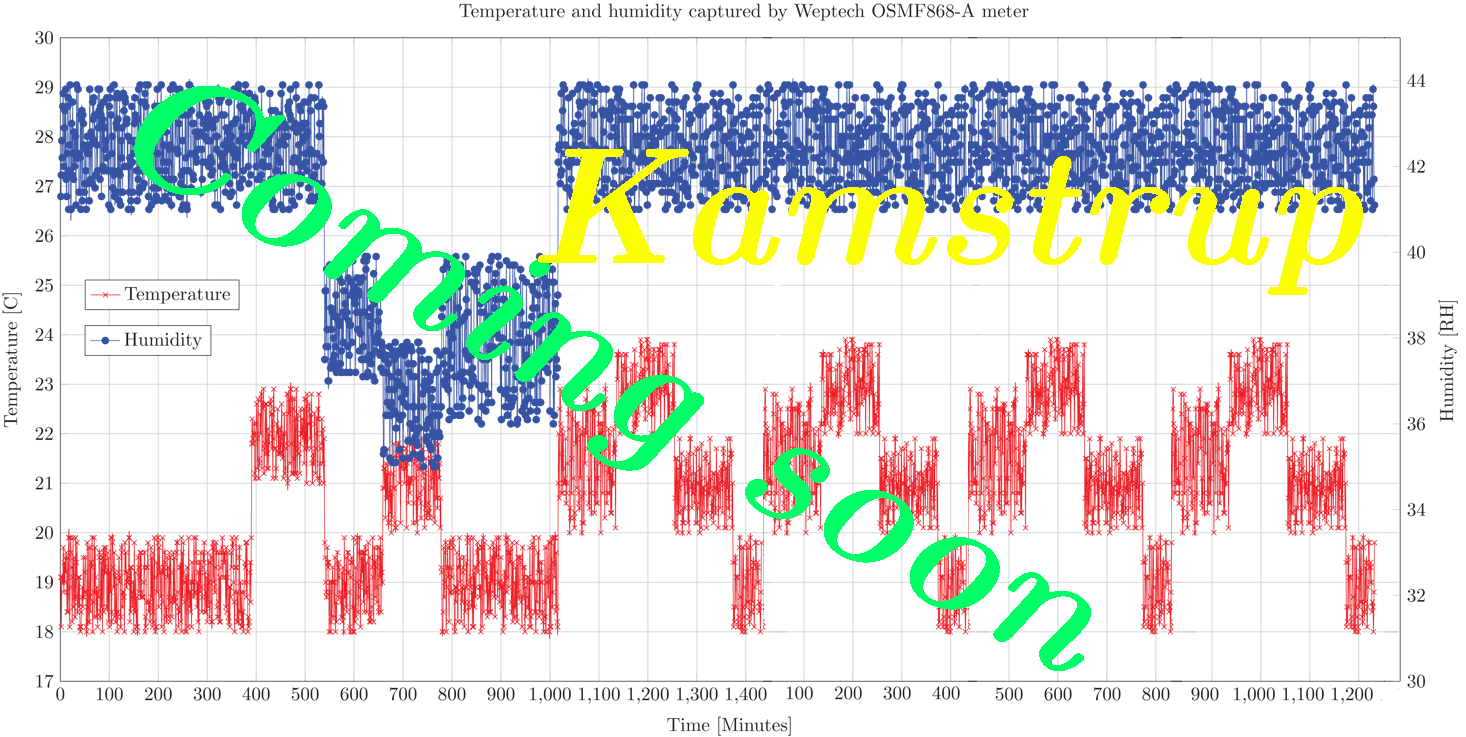
\includegraphics[scale=1.8]{obrazky/chart_kamstrup}
  \end{center}
  \caption{Vizualizace měření měřičem Kamstrup}
	\label{GrafPriloha4}
\end{figure}
\end{landscape}

%%%%%%%%%%%%%%%%%%%%%%%%%%%%%%%%%%%%%%%%%%%%%%%%%%%%%%%%%%%%%%%%%%%%%%%%%%%%%%%%%%%%%%%%%%%%%%%%%%%%%%%%%%%%%%%
\chapter{Obsah přiloženého DVD}
\label{PrilohaMedium}
K diplomové práci je přiloženo CD, obsahující bitový obraz MicroSD karty se systémem Raspbian, ve kterém je nainstalováno a nastaveno vše potřebné ke spuštění vzorové aplikace a zahájení komunikace s vyčítanými Wireless M-Bus zařízeními. Taktéž jsou zde uloženy zdrojové kódy vyčítačí i vizualizační aplikace.

\vspace{10pt}
Médium obsahuje následující strukturu: 
\vspace{-20pt}
	 \begin{figure}[!h]
  \begin{center}
    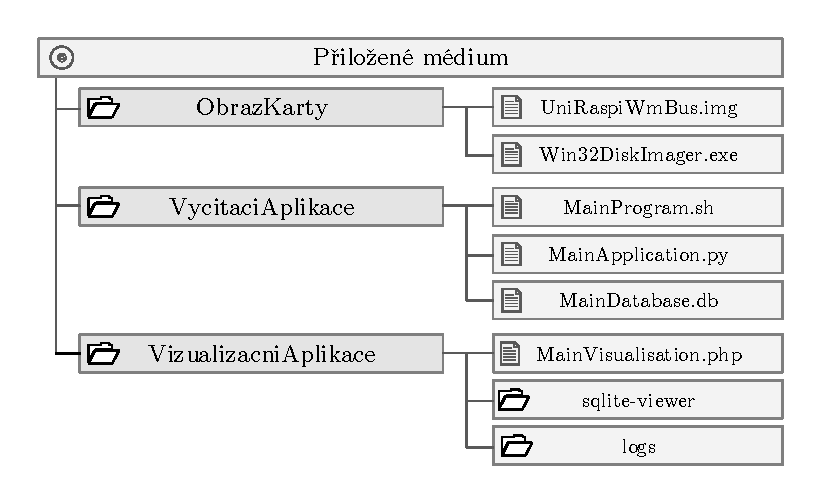
\includegraphics[scale=0.8]{obrazky/priloha_medium}
  \end{center}
	\vspace{-30pt}
\end{figure}

Návod pro spuštění aplikace:
		\begin{enumerate}
			\item Pomocí aplikace Win32DiskImager z \texttt{$\backslash$ObrazKarty$\backslash$Win32diskimager.exe} zapište obraz \texttt{$\backslash$ImageKarty$\backslash$UniPiRaspiWmBus.img} na pamětovou kartu typu MicroSD minimální velikosti 4GB.
			\item Kartu zasuňte do jednotky UniPi Neuron a zapněte tuto jednotku. Po startu jednotky dojde k aktivaci aplikace a zachytávání WM-Bus komunikace.
			\item Jednotka očekává přidělení IP adresy z DHCP serveru. Po přidělení IP adresy lze provádět vizualizaci zachytávaných dat pomocí aplikace na adrese \texttt{http:$\backslash$$\backslash$ip-adresa-jednotky$\backslash$}
			\item Případně po ssh přihlášení [\texttt{pi$\backslash$raspberry}] a zadání příkazu \texttt{screen -r} lze sledovat přímo výstup aplikace v konzoli.
		\end{enumerate}

	\vspace{10pt}
Vyčítací aplikace může být spuštěna samostatně, bez přítomnosti RaspberryPi, rozšiřující desky UniPi či IQRF komunikačního modulu. Je implementován demostrační režim s předpřipravenou sadou zachycených telegramů:
\begin{itemize}
	\item Režim příjmu zašifrovaných telegramů modulem IQRF: 
		\newline 
		\texttt{python MainApplication.py aes\_iqrf}
	\item Režim příjmu zašifrovaných obecných telegramů: 
		\newline 
		\texttt{python MainApplication.py aes\_clean}
	\item Režim příjmu nešifrovaných telegramů: 
		\newline 
		\texttt{python MainApplication.py clean}
\end{itemize}


